% !TEX root =  ../main_iclr.tex
In this work we propose a novel generative model for modeling the reaction mechanism of a subset of reactions with \emph{linear electron flow}.


\begin{figure*}[t!]
\centering
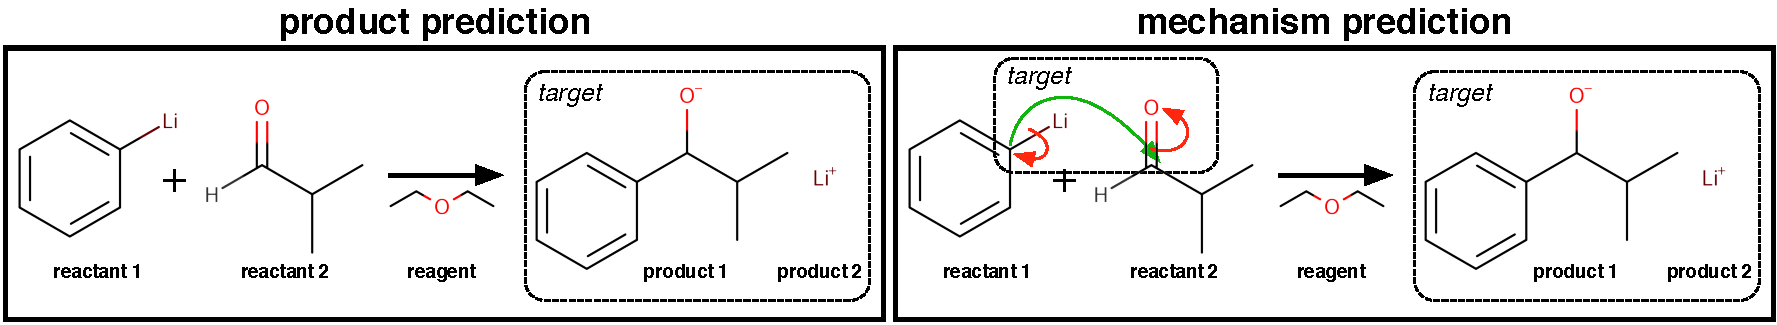
\includegraphics[width=\textwidth]{reaction_diagram.pdf}
\caption{\emph{(Left)} The reaction product prediction problem: Given the reactants and reagents, predict the structure of the product. \emph{(Right)} The reaction mechanism prediction problem: Given the reactants and reagents, predict how the reaction occurred to form the products.}
\label{fig:task-overview}

\end{figure*}
In Figure~\ref{fig:task-overview} we show the two challenges we tackle in this paper. 
On the left is \emph{product prediction}, where the goal is to predict the reaction products, given a set of reactants and reagents. However, for this task we do not care {\em how} the reactants react. For this, we also consider the task of \emph{mechanism prediction}, shown on the right. In this section, we begin by describing related work on these two problems, and then describe how a subset of reactions can be modeling by a single linear flow of electrons. In Section 3, we describe our generative model for predicting these reactions.



We argue that there are a number of benefits of predicting electron paths over predicting the outcomes of reactions directly (as is done in previous work \cite{jin2017predicting,schwaller2017found}):
\begin{itemize}
\item \textbf{Easy to interpret}: If the model makes a mistake, it is easy to see where, and possibly why, it goes wrong by comparing the steps of the path with the correct steps.
\item \textbf{Sparse}: Reactions often only affect between 3 and 7 atoms out of anywhere from 10-50 reactant atoms. Modeling the reaction as a path allows us to exploit this sparsity.
\item \textbf{Chemically consistent}: Learning a path allows us to easily incorporate chemical constraints, such as the alternating removal and addition of bonds, among others. 
\item \textbf{Generalizable}: As reaction paths follow similar trends in different molecules, our model naturally generalizes to unseen molecules. 
\end{itemize}





\vspace{-0.15cm}
\paragraph{Molecules and Chemical reactions.}


Organic molecules (those involving predominantly carbon) can be modeled as a graph structure, where each node is an atom and each edge is a covalent bond.
Covalent bonds represent 
one or more pairs of electrons that are shared between the atoms connected by the bond. 


Just as electrons describe the current structure of molecules, 
they also describe how molecules react with other molecules to produce new ones. All chemical reactions involve the stepwise movement of electrons along the atoms in a set of reactant molecules. 
This movement causes the formation and breaking of chemical bonds that changes the reactants into a new set of product molecules \citep{herges1994coarctate}. 
%
Reaction mechanisms can be classified by the topology of their "electron-pushing arrows". Here, the class of reactions with linear electron flow topology is by far the most important, followed by those with cyclic topology \citep{herges1994coarctate}. In this work, we will only consider reactions with linear topology that involve the movement of pairs of electrons.


%\vspace{-0.15cm}
\paragraph{Reactions as single electron paths.}
If reactions fall into this class, then a chemical reaction can be modeled as pairs of electrons moving in a \emph{single path} through the reactant atoms. 
Further, this electron path will alternately remove existing bonds in molecules, and form new ones. We show this alternating structure in the right hand part of Figure \ref{fig:task-overview}. 
The reaction formally starts by taking the pair of electrons between the Li and C atoms and moving them to the C atom (step 1); this is a remove bond step. 
Next comes an add step where electrons are moved from the C atom to form a bond between the two reactant molecules (step 2).
Then a pair of electrons are removed between the C and O atoms and moved to the O atom, giving rise to the products (step 3). 
Predicting the final product is thus a byproduct of predicting this series of electron steps.



